\chapter{Methods}\label{chap:methods}
LM converges to a stationary point of the cost function, and which stationary point it reaches is determined by where it begins. So, how do we get into the right basin?

The solver is only as good as its initial guess. This chapter builds a NN based initialiser which then provides an initial guess for LM to allow it to converge to the correct stationary point. 

In this chapter, we follow a pipeline. First we figure out how to sample poses uniformly in $\Omega$. Then, these poses are fed into the forward model, yielding eight measuremnts. These 8 measurements are passed to a solver which gives back a predicted pose. The pipeline is shown in Figure \ref{fig:model_pipeline}. The first two stages of the pipeline exist only at training time. At inference time, the system only executes the three remaining stages.

Section \ref{sec:datagen} implements the forward map from Section \ref{sec:forward-map} in Python and shows how to sample poses uniformly. Section \ref{sec:error} defines the positional and angular errors used to evaluate the solvers. Section \ref{sec:methods-lm} describes the LM solver, and shows implementation considerations. Section \ref{sec:representation} examines how the pose should be represented as a target, particularly with respect to angle. Section \ref{sec:network} describes the architecture and training of the NN solver. Section \ref{sec:hybrid} joins the two halves. 


\begin{figure}
  \centering 
  \includegraphics[width=0.8\textwidth]{figs/model_pipeline.png}
  \caption{Pose estimation pipeline.}
  \label{fig:model_pipeline}
\end{figure}
\section{Data generation}\label{sec:datagen}

\subsection{Anser Simulation in Python}
We simulate the Anser system in Python, developing on a MATLAB simulation by Jaeger et al. \cite{jaeger2017}. \footnote{The implementation is available at
\url{https://github.com/pmccarthy3901/ansermodelling}. A mapping from the
sections of this chapter to the corresponding modules is given in
Appendix~\ref{app:code}.}
The forward model proceeds as follows:

\paragraph{Coil geometry}
First we generate the vertex coordinates for a square spiral PCB emitter coil. This is done in a local coordinate system and then copies are rotated and translated to place them in the global coordinate system. 

Each coil is a square which spirals in, it has $N$ turns per layer, the sidelength of the outermost square is $l$, the trace width is $w$, there is a line to line spacing of $s$ and the thickness of the PCB is $z_\mathrm{thick}$. After the coil has done $N_{\mathrm{turns}}$ turns on the upper layer, it is connected with a via to the lower layer where the coil spirals out again. 

\paragraph{Conversion from Local to Global Coordinates}
As all of the coils are the same shape, only one coil is generated, then it is copied a number of times into different places in space. 
The module selects an axis about which the rotation takes place. This is represented as an integer $(0,1,2) - (x,y,z)$. This works nicely because the rotation matrix can be generated using an even permutation of the axes. The module then applies the permuted rotation matrix to a copy of the input vector and then applies a translation.

\paragraph{Field Calculation}
The calculation of the magnetic field generated by the coils is done in \lstinline[style=python]|field_coil_calc|. It uses the linearity of the Biot-Savart line integral to calculate the total magnetic field due to the coils at an observer point as the sum of the contributions of each straight-line segment. It then implements equation \eqref{eq:biot_savart_final} to calculate the magnetic field.

%/\paragraph{Objective Function}

%The objective function \eqref{eq:objective_function} takes in the real observed measurement, and returns the difference between it and the measurement calculated using the simulation. It calculates the simulated measurement as:

%\begin{equation}
%  \mathbf{m}_\mathrm{sim} = \mathbf{H}_\mathrm{sim} \cdot \hat{n}_\mathrm{obs}
%\end{equation}
%where:
%\begin{itemize}
%  \item $\mathbf{H}_\mathrm{sim}$ is the simulated magnetic field 
%  \item $\hat{n}_\mathrm{obs}$ is the unit vector along the sensor axis.
%\end{itemize}
%Then, the objective function is calculated as: 
%\begin{equation}
%  \mathbf{r}:= \mathbf{m}_{\mathrm{sim}} - \mathbf{m}_{\mathrm{obs}}
%  \label{eq:objective_function}
%\end{equation}


\subsection{Sampling}
When generating data, it is important that our sampling space is uniform. For position, this is easy, we sample uniformly in the bounds of the box. The angle, however requires a bit more consideration.

\subsubsection{Sampling the position}
The Anser system operates in a 25x25x25cm box. 

Since the sensor coil is on a PCB that is $1.6$mm thick, the $z$ value has a minimum of $z = 0.0016$m. Therefore we sample uniformly within the bounds shown in Table \ref{tab:pos_bounds} 

\begin{table}
  \centering
  \begin{tabular}{lcc}
    \toprule
    Variable & Min (mm) & Max (mm) \\
    \midrule
    $x$ & $-125$ & $125$ \\
    $y$ & $-125$ & $125$ \\
    $z$ & $1.6$ & $250$ \\
    \bottomrule
  \end{tabular}
  \caption{Bounds of the sampling volume.}
  \label{tab:pos_bounds}
\end{table}
\subsubsection{Sampling the orientation}

Consider an area element $dA$ on the unit sphere, seen in Figure \ref{fig:unit_sphere}. Then the area element is $d A = \sin\theta d \theta d \phi$. Therefore, to uniformly sample on the sphere we must not sample uniformly in $\theta$, but rather in $\cos \theta$. The orientation sampling is shown in Table \ref{tab:angle_bounds}. As seen in Figure \ref{fig:orientation_sampling}, this leads to uniform sampling on the sphere. 

\begin{figure}
  \centering
  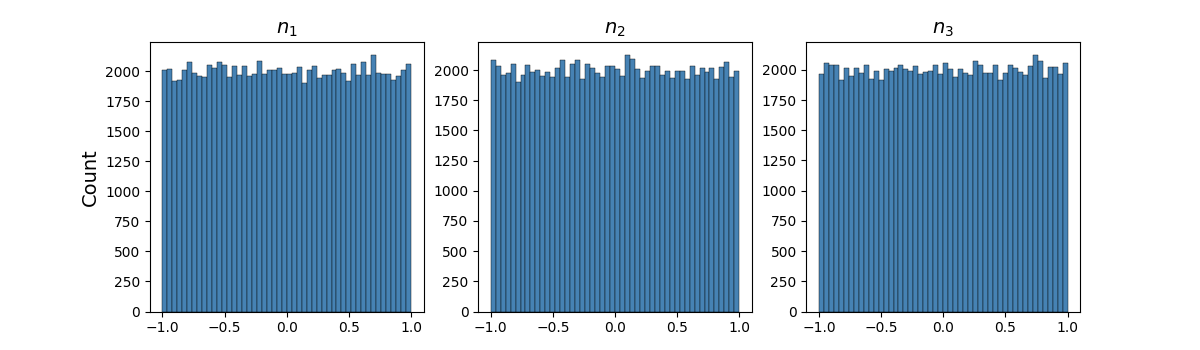
\includegraphics[width = 0.8 \textwidth]{figs/orientation_sampling.png}
  \caption{Orientation normal vectors sampled.}
  \label{fig:orientation_sampling}
\end{figure}

\begin{table}
  \centering
  \begin{tabular}{lcc}
    \toprule
    Variable & Min & Max \\
    \midrule
    $\cos\theta$ & $-1$ & $1$ \\
    $\phi$ & $0$ rad & $2\pi$ rad \\
    \bottomrule
  \end{tabular}
  \caption{Bounds of the orientation sampling volume.}
  \label{tab:angle_bounds}
\end{table}

\begin{figure}
  \centering
  \includegraphics[width = 0.4\textwidth]{figs/unit_sphere.png}
  \caption{Area element on the unit sphere. Reproduced from \cite{secil2023}}
  \label{fig:unit_sphere}
\end{figure}

\subsection{Dataset size, split, and normalisation}
The dataset consists of pose-measurement pairs. A subset of the poses are shown in space in Figure \ref{fig:sampled_poses}. The measurements are the model input and the pose is the regression target. The data is split 80/20 into training and validation sets, and the validation set is never seen during training. Models are then evaluated on a held out test set. The distribution of datapoints is shown in Table \ref{tab:data_splits}

\begin{table}
  \centering
  \begin{tabular}{ll}
    \toprule
    Split & Size \\
    \midrule
    $N_{\mathrm{train}}$ & $80,000$ \\
    $N_{\mathrm{val}}$ & $20,000$ \\
    $N_{\mathrm{test}}$ & $20,000$ \\
    \bottomrule
  \end{tabular}
  \caption{Data splits between training, validation, and testing data.}
  \label{tab:data_splits}
\end{table}
  

\begin{figure}
  \centering 
  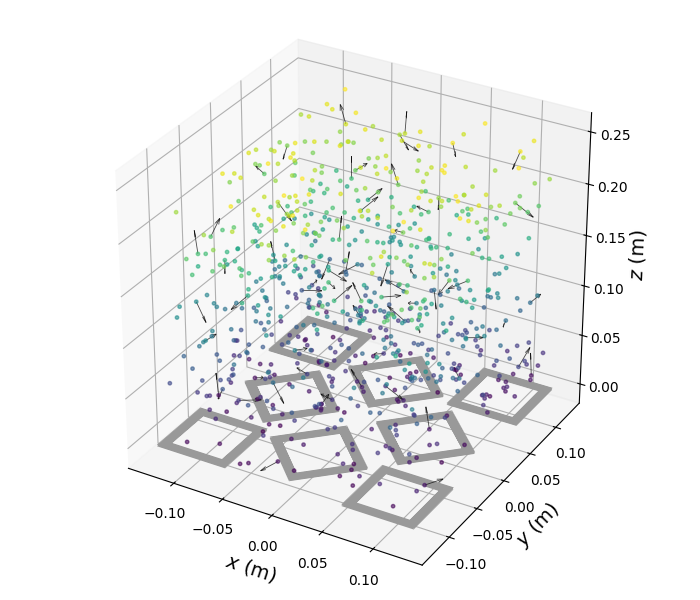
\includegraphics[width = 0.8 \textwidth]{figs/sampled_poses.png}
  \caption{800 poses sampled with some arrows indicating orientation.}
  \label{fig:sampled_poses}
\end{figure}

\section{Error metrics}\label{sec:error}
In order to quantify how "good" a particular model is, we need to define our errors. Since the pose has two components: position and orientation, we define an error on each. 

\subsection{Positional Error}
The positional error $e_p$ is defined using the euclidean distance between the true position, $x_\mathrm{true}$, and the predicted position, $x_\mathrm{pred}$.
\begin{equation}
  e_{p} := \left\Vert x_\mathrm{true} - x_\mathrm{pred} \right\Vert_2
\end{equation}

\subsection{Angular Error}
The angular error, $e_{\hat{n}}$, is defined in relation to the unit normal orientations, where $\hat{n}_\mathrm{true}$ is the true unit normal, and $\hat{n}_\mathrm{pred}$ is the predicted unit normal:
\begin{equation}
  e_{\hat{n}} := \arccos \left( \hat{n}_\mathrm{true} \cdot \hat{n}_\mathrm{pred} \right)
\end{equation}

\section{The Levenberg-Marquardt solver}\label{sec:methods-lm}
The previous chapter derived the LM update function \eqref{eq:lm}. This section describes the implementation and parameter choice. The chosen parameters were tuned against the validation set and are shown in Table \ref{tab:lm_parameters} 

\begin{table}
  \centering
  \begin{tabular}{ll}
    \toprule
    Property & Value \\
    \midrule
    $\lambda_0$ (Initial damping) & $10^{-5}$ \\
    $\lambda_{\max}$ (Maximum damping) & $10{^7}$ \\
    $\epsilon_{\mathrm{grad}}$ (Gradient threshold) & $10^{-5}$ \\
    Maximum Iterations & $100$ \\
    $h$ (Jacobian finite difference) & $10^{-5}$ \\
    \bottomrule
  \end{tabular}
  \caption{Parameters used in LM implementation.}
  \label{tab:lm_parameters}
\end{table}

\subsection{Implementation}
The solver is implemented in NumPy (\lstinline[style=python]|models/LM_solve.py|). Its components are as follows:

\paragraph{Jacobian.} As discussed in the previous chapter, we approximate the Jacobian using finite difference, as in \eqref{eq:jacobian}.

\paragraph{Scaling.} Following Marquardt's implementation \cite{marquardt1963}, the damping matrix is given by:
\begin{equation}
  D = \text{diag}(\max(\text{diag}(J^\top J), 10^{-12}))
\end{equation}
where the floor of $10^{-12}$ guards against a zero diagonal entry making $D$ singular and $\text{diag}$ is the function defined in Section \ref{sec:background-lm}

\paragraph{Constraint Handling.} At each iteration, constraints are applied to both the position and orientation. The position is clipped to within the box shown in Table \ref{tab:pos_bounds}. The orientations are handled by folding $\theta$ through the pole with a $\pi$ shift in $\phi$, and wrapping $\phi$. This keeps the orientation unchanged on the unit sphere and alters only its coordinates.

\paragraph{Damping.} Damping is done as in Section \ref{sec:background-lm}.

\paragraph{Stopping.} Iteration terminates when any of three conditions are met:
\begin{enumerate}
  \item the $l_{\infty}$ norm of the gradient falls below a threshold, $\epsilon_{\mathrm{grad}}$.
  \item The damping parameter, $\lambda$ exceeds $\lambda_{\mathrm{max}}$, indicating that no downhill step can be found. 
  \item A maximum number of iterations is reached, indicating that the solver cannot find a solution.
\end{enumerate}
Only the first of those three stopping criteria indicates success, and even then, the solver successfully reaching a minimum does not mean that it has successfully reached the correct minimum. Therefore we have to define convergence.

We say that a solution has converged if for some $\epsilon_p$ and some $\epsilon_n$ "acceptable errors":
\begin{align*}
  e_p &< \epsilon_p \\
  e_{\hat{n}} &< \epsilon_n 
\end{align*}

\section{Representing the pose}\label{sec:representation}
The pose contains two angles, and how they are represented as regression targets matters more than it first appears. Regressing against $\theta$ and $\phi$ directly has three problems. First, $\phi$ is periodic: $\phi = 0.01$ and $\phi = 2\pi - 0.01$ are only separated by $0.02$ rad, however a naive loss would heavily punish such a situation. The second problem is with $\phi$: at the poles $\theta \in \{0,\pi\}$, $\phi$ is not defined. The third problem is more general: squared error in the angles is not a distance on the sphere. The metric induced on the unit sphere, $S^2$, by the parametrisation carries an extra factor of $\sin^2\theta$:
\begin{equation}
  ds^2 = d\theta^2 + \sin^2\theta \, d\phi^2 
\end{equation}

For these reasons, it becomes natural to represent the orientation not in terms of angles, but in terms of the unit normal itself:

\begin{equation}
  \hat{n}(\theta,\phi) = \begin{bmatrix} \sin\theta\cos\phi \\ \sin\theta\sin\phi \\ \cos\theta \end{bmatrix}
\end{equation}
The normal vector is smooth, unique, and has no wrap-around. We therefore train networks whose target is the vector:
\begin{equation}
  t = (x,y,z,n_1,n_2,n_3)
\end{equation}
where $n_i$ is the unit normal in the $i$th direction.

This argument, however, does not apply to the LM solver of Section \ref{sec:methods-lm}, which continues to operate in the $(\theta,\phi)$ regime. This is because an iterative solver initialised near its solution does not encounter these problems and, conversely, if we were to regress against the unit normal we would have the issue of having 6 parameters for 5 degrees of freedom meaning that $J^{\top} J$ would not be invertible, contradicting the exact condition that LM needs.  


\section{Neural Network Solver}\label{sec:network}
Section \ref{sec:methods-lm} establishes that the LM solver needs a good initial guess to converge. This section builds a NN solver, the main advantage of which is its ability to learn the global configuration of the system and thus work on a "cold start". This section shows the choice of architecture, loss function, and training methods.
\subsection{Neural Network Architecture}
The NN solver uses a basic feed-forward-neural-network which takes the 8 input measurements and outputs the 6 dimensional pose $(x,y,z,n_1,n_2,n_3)$. The NN architecture is shown in Table \ref{tab:architecture} 

\begin{table}
  \centering
  \begin{tabular}{ll}
    \toprule
    Property & Value \\
    \midrule
    Input dimension       & 8 (measurements) \\
    Output dimension      & 6 ($x, y, z, n_1, n_2, n_3$) \\
    Hidden layers         & 3 \\
    Units per layer       & (256,256,256) \\
    Activation            & tanh \\
    \bottomrule
  \end{tabular}
  \caption{Network architecture.}
  \label{tab:architecture}
\end{table}
\subsection{Choice of loss function}\label{sec:methods-loss}
In Section \ref{sec:error} we defined two errors: $e_p$, the positional error, and $e_{\hat{n}}$, the angular error. Now we must define a loss function. The only problem is that these errors operate on completely different scales. Given the bounds of our box, $e_p$ varies between $0$ and $w_p$, where $w_p$ is the diagonal length of the box, and $e_{\hat{n}}$ varies between $0$ and $w_{\hat{n}} = \pi$. To give equal weight to both components we define our loss, $\mathcal{L}$, as the weighted sum between squares of the two as follows: 
\begin{equation}
  \mathcal{L} = e_p^2 + \frac{w_p^2}{w_{\hat{n}}^2} e_{\hat{n}}^2
  \label{eq:loss}
\end{equation}
This weight is chosen such that the two terms have equal range over the sampling volume.
\subsection{Neural Network Training}
The network is trained with the Adam optimiser \cite{kingma2017} to minimise \eqref{eq:loss} over the dataset described in Section \ref{sec:datagen}, using the settings and hyperparameters described in Table \ref{tab:training}

The learning rate uses a cosine scheduler \cite{loshchilov2017}, decaying from its initial value to zero, as in equation \eqref{eq:cosine_annealing} with parameters in Table \ref{tab:training}, where $t$ is the current epoch and $\eta_0$ is the learning rate at the 0th epoch. This allows for a high learning rate at the start, which then decays smoothly at every epoch. This means that at the start the model learns quickly, and at the end the model has sufficiently small learning rate to not oscillate around the minimum. 

\begin{equation}
  \eta_{t+1} = \eta_{\mathrm{min}} + (\eta_t - \eta_{\mathrm{min}}) \frac{1 + \cos \left( \frac{t+1}{T_{\mathrm{max}}}\pi \right)}{1 + \cos \left( \frac{t}{T_\mathrm{max}} \pi \right)}
 \label{eq:cosine_annealing} 
\end{equation}
\begin{table}
  \centering
  \begin{tabular}{ll}
    \toprule
    Parameter & Value \\
    \midrule
    Optimiser       & Adam \\
    Schedule        & Cosine Annealing \\
    Batch size      & 32 \\
    Epochs          & 200 \\
    $\eta_{0}$ & $10^{-3}$ \\
    $\eta_{\mathrm{min}}$ & $0$ \\
    $T_{\max}$ & $200$ \\
    \bottomrule
  \end{tabular}
  \caption{Training configuration.}
  \label{tab:training}
\end{table}
\section{Hybrid Model}\label{sec:hybrid}
Sections \ref{sec:methods-lm} and \ref{sec:network} present a LM based solver and a NN solver, respectively. The shortcomings of these two solvers are complementary. A hybrid model combines these two, feeding the output of the NN model into a LM solver. This allows the NN to provide a good initialisation for the LM solver to further refine.

\subsection{Coupling the two solvers}
The two components operate in different parametrisations. The NN uses $(x,y,z,n_1,n_2,n_3)$ and the LM solver uses $(x,y,z,\theta,\phi)$. This means that before feeding the NN output into the LM solver, we have to convert the parametrisation.

Given the predicted normal $\hat{n} = (n_1,n_2,n_3)$, normalised to unit length, the corresponding $\theta$ and $\phi$ are given by: 
\begin{align*}
  \theta &= \arccos(n_3) \\
  \phi &= \operatorname{atan2}(n_2,n_1)
\end{align*}
where $\operatorname{atan2}$ is the two argument arctangent defined by:
\begin{equation}
  \operatorname{atan2}(y,x) =
  \begin{cases}
    \arctan\!\left(\frac{y}{x}\right)         & \text{if } x > 0, \\
    \arctan\!\left(\frac{y}{x}\right) + \pi   & \text{if } x < 0 \text{ and } y \geq 0, \\[6pt]
    \arctan\!\left(\frac{y}{x}\right) - \pi   & \text{if } x < 0 \text{ and } y < 0, \\[6pt]
    +\frac{\pi}{2}                            & \text{if } x = 0 \text{ and } y > 0, \\[6pt]
    -\frac{\pi}{2}                            & \text{if } x = 0 \text{ and } y < 0, \\[6pt]
    \text{undefined}                          & \text{if } x = 0 \text{ and } y = 0.
  \end{cases}
  \label{eq:atan2}
\end{equation}
The use of $\operatorname{atan2}$ instead of the normal arctangent allows us to both get in the correct quadrant and also mitigates against the singularity caused when $n_1 = 0$.

Now we can build our hybrid pipeline. The pipeline is shown in Figure \ref{fig:hybrid_pipeline}

\begin{figure}
  \centering 
  \includegraphics[width = 0.8 \textwidth]{figs/hybrid_pipeline.png}
  \caption{Data pipeline for hybrid model}
  \label{fig:hybrid_pipeline}
\end{figure}
